% METODOLOGIA

\chapter{SISTEMA DE ATUALIZAÇÃO DE FIRMWARE OVER-THE-AIR}
\label{chap:metodologia}
Nesse capitulo é retratado como é o funcionamento do sistema que será desenvolvido, mostrando inicialmente uma visão geral do projeto, como o conjunto de firmwares (OTA e \bootloader) funcionam em conjunto para executar a atualização da aplicação. São listadas as funcionalidades de cada uma das partes do \textit{software}, explicando suas atividades e a forma com que foram implementadas, como cada biblioteca foi utilizada nestas aplicações. Aqui também são apresentados quais os materiais utilizados, e quais os \textit{firmwares} criados para a prova de que o sistema funciona, e uma explicação de como utilizar o sistema desenvolvido neste trabalho em outras plataformas embarcadas da familia de microcontroladores STM32.

\section{VISÃO GERAL}
O \textit{software} que foi desenvolvido nesse trabalho é dividido em duas partes, um \bootloader, e uma API para implementar um cliente OTA. O \bootloader, com o auxílio da biblioteca FatFs, realizará a comunicação com o cartão SD, que conterá a última versão do \firmware\ previamente recebido. Assim poderá substituir o \software\ anterior da aplicação por um novo. Essa parte do \software\ ficará armazenada em uma região da memória que dificilmente será reescrita, podendo ser reescrita somente com o auxílio de ferramentas de desenvolvimento como um JTAG e/ou \textit{debugger}, então é uma peça do programa que improvavelmente será substituída. Será uma parte que é portável para todos os microcontroladores da familia STM32, pois faz uso direto de funções de escrita na memória flash obtidas por meio do STM32Cube HAL, ficando a cargo do projetista fazer uma pequena adaptação, que posteriormente será explicado neste trabalho.

A API para o cliente OTA contêm as funções necessárias para se comunicar com um servidor e fazer a busca pela versão mais atual do \firmware, bem como para fazer o \textit{download} dessa nova versão do \firmware\ para um cartão SD. Para tanto, são utilizadas as bibliotecas LwIP que implementa o protocolo TCP/IP, a biblioteca MbedTLS que implementa o protocolo de criptografia e autenticação TLS e, a biblioteca FATFs para a leitura e escrita do cartão SD.

Após ser confirmada a existência de uma nova versão de \firmware, o cliente OTA irá se comunicar novamente com o servidor com o intuito de fazer o \download\ dessa nova versão, e a armazena no cartão SD do sistema. Com o \download\ concluído com sucesso, a API é utilizada novamente para obter do servidor o arquivo contendo o hash deste \firmware. Após o cliente OTA executa uma função que cria o hash do \firmware\ baixado anteriormente e o compara com o arquivo hash obtido do servidor. Para assim garantir que o \firmware\ está integralmente e não corrompido no cartão SD. Finalmente, ao confirmar um novo firmware válido, é gerado uma reinicialização do sistema. Na inicialização, o \bootloader\ é executado para a troca de \firmware. O funcionamento mais detalhado do \bootloader\ e da API de atualização OTA explanada ainda neste trabalho, mas de forma geral a sequência de operação é descrita no fluxograma apresentado na \autoref{fig:visaogeral}.



\begin{figure}[H]
    \scriptsize
     \centering
     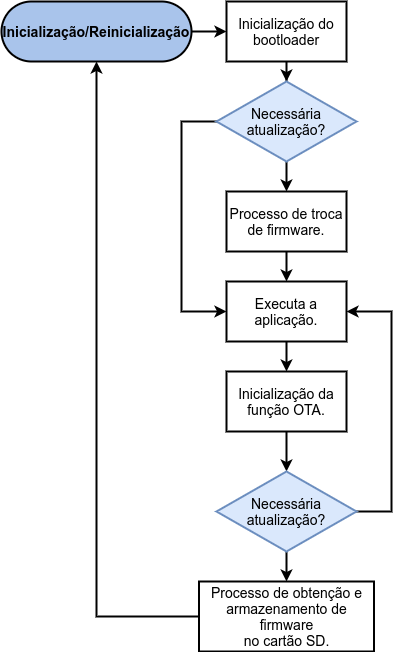
\includegraphics[scale=0.7]{dados/figuras/FuncionamentoGeral.png}
     \caption{Visão geral do funcionamento do sistema de atualização. \newline Fonte: autoria própria.}
     \label{fig:visaogeral}
\end{figure}

A API será uma peça de \software\ que poderá ser substituída e atualizada em conjunto com as demais aplicações do sistema, como, as bibliotecas LwIP, MbedTLS, o sistema operacional, entre outras peças de \software\ utilizadas pela aplicação. 
O sistema de atualização OTA utiliza-se de bibliotecas já conhecidas e vastamente utilizadas por desenvolvedores de sistemas embarcados. Assim projetos que necessitem fazer comunicação segura via rede, leitura e escrita de cartões SD, possam utilizar esse sistema de modo a poupar espaço na memória, visando a reutilização dessas bibliotecas. Portanto, o sistema pode ser amplamente utilizado por sistema de IoT. 
%Será utilizada o \textit{kit} de desenvolvimento STM32F746G \textit{Discovery}, onde será inicialmente desenvolvida a API, suas tarefas e o \textit{bootloader} que serão os principais componentes desse sistema.

Em caso de uma falha durante o processo de atualização OTA, o sistema tem a habilidade de se recuperar de forma autónoma. Como não haverá sobrescrita na área em que o \textit{firmware} está posicionado no cartão SD, uma simples reinicialização do sistema pode fazer com que o \bootloader\ seja ativado novamente e refaça o processo de cópia da memória.

É importante lembrar que o armazenamento do \firmware\ e demais arquivos com informações para o processo de atualização poderia ser feito em qualquer mídia de armazenamento presente no sistema embarcado que se deseja utilizar. Seria possível por exemplo, utilizar a o espaço restante da memória flash para armazenar esses dados, uma memória EEPROM, ou mesmo os 128 Mbits de memória Quad-SPI flash presentes no kit de desenvolvimento utilizado para teste neste projeto, Por definição de projeto desse trabalho foi selecionado o cartão SD para esse armazenamento.
%O sistema de atualização irá funcionar da seguinte forma, após a inicialização do sistema o \bootloader\ é executado e verifica a existência de um novo \firmware, no caso negativo ele inicia normalmente o \software\ principal da aplicação. No caso positivo, o \bootloader\ inicia o processo de substituição de \textit{firmware}, após a troca, o novo \software\ é iniciado. Durante a execução da aplicação principal do sistema e em um tempo determinado pelo projetista, a API entra em contato com o servidor para verificar a disponibilidade de um \software\ novo, em caso positivo ela agenda um período para a atualização do \firmware, no caso negativo ele continua a execução da aplicação. 

%Caso haja uma atualização quando o horário do agendamento chegar, a API irá conectar-se ao servidor e iniciar o processo de \download\ do \firmware\ novo e armazená-lo em uma área já predefinida do cartão SD para que o \bootloader\ possa o encontrar. Após o \download\ o sistema será reiniciado e o \bootloader\ entrará será executado novamente. 
%De forma resumida o funcionamento do sistema pode ser visto na \autoref{Funcionamento}, 


%Com a  As tarefas serão produzidas a partir de b
%sistema possa conter intersecções com trechos de codigos utilizados em varios projetos que necessitam

%Adicionar diagrama de blocos!!!!

% A seguir será explicado parcialmente como funcionarão as funções das tarefas, do \textit{bootloader}, e do servidor HTTP.
%Cada capítulo deve conter uma pequena introdução (tipicamente, um ou dois parágrafos) que deve deixar claro o objetivo e o que será discutido no capítulo, bem como a organização do capítulo.

\section{\textit{BOOTLOADER}}
\label{sec:Bootloader}

A partir de um arquivo de \textit{linker}, a memória da plataforma será customizada com o intuito de abrigar os arquivos necessários para o \bootloader\ e protegê-lo de eventuais sobrescritas que podem vir a ocorrer. Esse arquivo de \textit{linker}, assim como o próprio \textit{bootloader}, será escrito somente para os microcontroladores da familia STM32, visto que cada plataforma tem suas próprias características como, tamanho de memória e endereços diferentes para cada fabricante e/ou arquitetura.

No arquivo de \linker\ será especificada uma área especial na memória flash do sistema em que será abrigado o \bootloader. Também será responsável por fazer com que o \bootloader\ seja chamado após a inicialização do sistema. Assim será garantido que o \bootloader\ sempre entre seja executado após a reinicialização do sistema embarcado.

%irá verificar o \textit{hash} da nova versão, verificando a integridade e origem do \textit{software},

O \textit{bootloader} será responsável em fazer a troca de cada versão de \textit{firmware} instalado no sistema embarcado. Sempre que o sistema for iniciado, o \textit{bootloader} será inicializado e fará a procura de arquivos. Essa busca será possível pelo fato da biblioteca FatFs, que está implementada junto ao \bootloader, criar um sistema de arquivos no cartão SD do sistema alvo, assim o \bootloader\ pode acessar a memória do cartão sem a necessidade da aplicação final ser inicializada.

Se após o \textit{reset} a procura do arquivo contendo a versão do \firmware\ novo retornar com um resultado positivo, ele converte o valor contido neste arquivo de uma string para um tipo inteiro e o compara com os quatro últimos bytes da memória flash, posição onde se encontra a versão atual do \firmware , caso a versão do novo firmware seja maior que a do firmware atual o \bootloader\ inicia o processo de atualização.

Nesse processo o \bootloader\ substitui completamente o \textit{firmware} e demais bibliotecas e API's em áreas não protegidas na memória, pelo binário do \textit{firmware} presente no cartão SD. Esse processo é implementado com o uso das funções de escrita na memória flash do HAL fornecido pela STM32, onde inicialmente é feito o processo de apagamento massivo dos setores da aplicação da memória flash, dessa forma esses setores são preenchidos com o valor 0xFF em cada byte.

Após o processo de apagamento é iniciado o processo de escrita, em que o arquivo contendo o \firmware\ é lido a cada 512 bytes para um buffer, e a partir deste buffer são escritos 4 bytes por vez na memória flash, assim esse processo se repete até que o arquivo contendo o novo firmware seja completamente escrito na memória.
Finalizada a escrita do novo \firmware, acontece a escrita do numero de versão nos quatro últimos bytes da memória, somente após essa escrita o processo de atualização pode ser considerado concluído com sucesso, e então ele pode apagar do cartão SD os arquivos do \firmware\ e versão.

Caso o \bootloader\ seja iniciado e em algum momento detectar que o valor dos quatro últimos bytes são iguais a 0xFFFFFFFF, ele identifica que a ultima operação de atualização não foi concluída com exito. Neste estado o \bootloader\ fica sempre tentando encontrar uma nova versão do \firmware\ no cartão SD e caso não encontre ele fica reiniciando o microcontrolador, e caso ele encontre, o \bootloader\ tenta atualizar novamente com o \firmware\ encontrado, independente da versão dele, garantindo assim que o sistema seja resistente a eventuais erros e eventos não previstos, como quedas de energia durante o processo. O funcionamento do \textit{bootloader} pode ser observado na \autoref{fig:DiagBootloader}.

\begin{figure}[H]
    \scriptsize
     \centering
     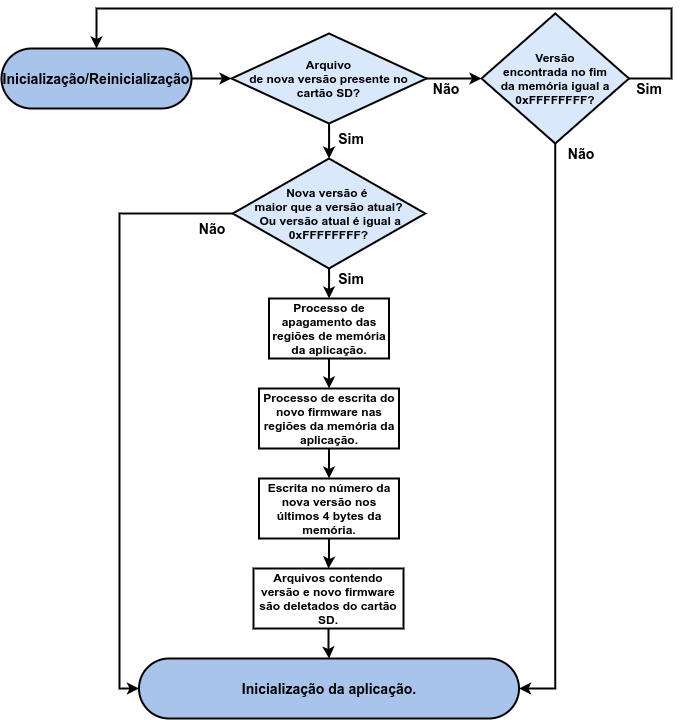
\includegraphics[scale=0.6]{dados/figuras/FuncionamentoBootloader.png}
     \caption{Diagrama de funcionamento do \bootloader. \newline Fonte: autoria própria.}
     \label{fig:DiagBootloader}
\end{figure}
%Inserir seu texto aqui...

%\section{SERVIDOR HTTP}
%\label{sec:ServidorHTTP}

%A partir de um computador conectado à mesma rede que o sistema embarcado, haverá um servidor HTTP que ficará responsável por esperar requisições do dispositivo, para consultar a disponibilidade de uma versão atualizada do \textit{software}, e após a confirmação dessa nova versão, esse servidor irá enviar o \textit{firmware} para a plataforma embarcada.
%Inserir seu texto aqui...

\section{API DE ATUALIZAÇÃO OTA}
\label{sec:API}

A API de atualização OTA que foi desenvolvida nesse trabalho tem o propósito de ser o mais portável possível, para assim, ser reutilizada por diversos projetos que necessitem da troca de seu \software\ e com isso pode ser chamada quando o desenvolvedor necessitar, como após uma interrupção externa ou comando do servidor. Com esse objetivo, serão utilizadas as bibliotecas já bem difundidas, a LwIP para a criação da pilha TCP/IP, a Mbed TLS para criar uma camada se segurança nessa pilha, e a FATFS para a criação de um sistema de arquivos FAT. Assim desenvolvedores podem se aproveitar do fato de que essas bibliotecas já estão em seus sistemas como padrão para utilizá-las em suas próprias funcionalidades. 
A seguir será retratado como serão cada uma das funcionalidades necessárias na API.

\subsection{COMUNICAÇÃO COM O SERVIDOR}

Com o uso da biblioteca LwIP e Mbed TLS foi criada uma pilha de comunicação no sistema alvo, que é responsável pela conexão segura com o servidor que fornecerá o novo firmware. Na implementação da pilha de comunicação, foi utilizada a API BSD Sockets, pois, o intuito é deixar o sistema de atualização portável, e essa API fornece suporte a sistemas operacionais de tempo real entre outra vantagens.

Como a biblioteca Mbed TLS já foi desenvolvida para ser integrada facilmente a várias aplicações embarcadas, ela foi utilizada para criar protocolos de segurança nessa comunicação com o servidor. Foram utilizados padrões SSL/TLS para ser criado um canal criptografado entre o servidor e o sistema alvo, para garantir que todos os dados transmitidos sejam sigilosos e seguros.

A comunicação com o servidor será feita por meio de um servidor HTTP que utilizará o protocolo TCP para garantir que todos os dados obtidos pelo servidor sejam integros, evitando que o novo \textit{firmware} e demais dados obtidos sejam corrompidos. 

%essa tarefa estará responsável por criar uma comunicação segura entre o \textit{hardware} e o servidor HTTP, a partir dessa comunicação será feito a verificação do sinal de disponibilidade de novo \textit{software} e \textit{download} do mesmo quando o sistema estiver ocioso. 

\subsection{DOWNLOAD E ARMAZENAMENTO DO FIRMWARE}

A partir da utilização da biblioteca FatFs, será criado um sistema de arquivo FAT, que gerenciará a memória presente no cartão SD dentro da aplicação, e ele pode ser utilizado tanto pela aplicação final do sistema embarcado, quanto pela API. Esse sistema de arquivo será utilizado para que se possa identificar a posição na memória em que o \textit{firmware} novo será colocado após o seu \download, evitando que outros arquivos, pertencentes a aplicação final, sejam colocados com o mesmo nome, e fazendo com que o \bootloader\ interprete de forma errada os arquivos gerando erros.

Quando o desenvolvedor iniciar a função OTA, a API iniciará novamente a comunicação com o servidor que contém a última versão do \textit{firmware}, dessa vez com o propósito de fazer \download\ do arquivo contendo o numero da nova versão do \textit{software}. Após o \download\ a API ainda irá verificar se o valor obtido por meio deste arquivo é maior que o presente nos últimos 4 bytes da memória, para assim verificar se existe a necessidade de se continuar com o processo de atualização. 

Caso o valor da nova versão seja maior que a versão atual do firmware a API inicia o \download\ do novo firmware, após esse processo a ferramenta inicia a comunicação novamente para obter agora o arquivo contendo o hash do firmware posteriormente baixado, e com isso é feito um teste de integridade neste firmware onde inicialmente se gera um hash a partir do algoritmo SHA-256 fornecido pela biblioteca MBED TLS, e esse hash é comparado com aquele baixado do servido. Se esse teste retornar com sucesso o processo de atualização é continuado, e o arquivo de hash baixado do servidor é apagado do cartão SD e é iniciado o processo de reinicialização do microcontrolador com o intuito de se iniciar o bootloader para completar o processo de atualização.
A \autoref{fig:DiagAPI} ilustra o funcionamento da API.

\begin{figure}[H]
    \scriptsize
     \centering
     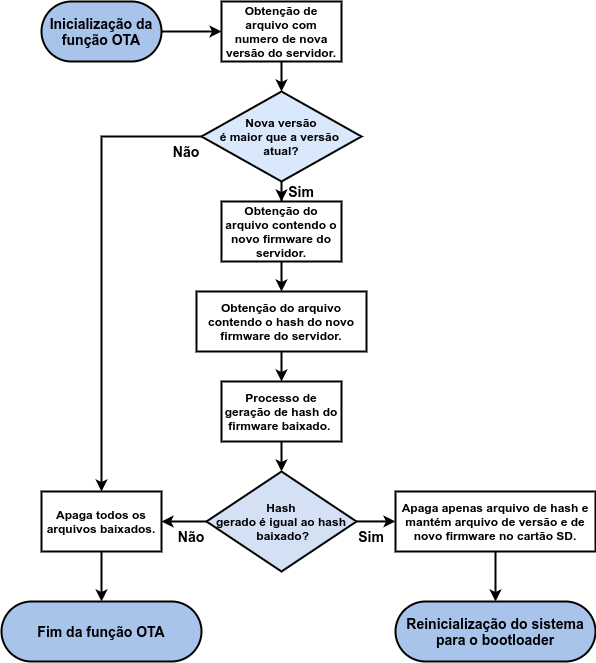
\includegraphics[scale=0.67]{dados/figuras/FuncionamentoAPI.png}
     \caption{Diagrama de funcionamento da API.\newline Fonte: autoria própria.}
     \label{fig:DiagAPI}
\end{figure}
%maquina de estado para leitura do arquivo.

\section{CRIAÇÃO DE FIRMWARE E ARQUIVOS PARA O SISTEMA DE ATUALIZAÇÃO}
Para a utilização do sistema de atualização OTA desenvolvido nesse trabalho é necessário que o \firmware\ e arquivos que serão disponibilizado no servidor mantenham um padrão determinado, assim está sessão explicará como dever ser feito o processo de criação destes arquivos e a criação do \firmware.

\subsection{CRIAÇÃO DE ARQUIVOS AUXILIARES}
Os arquivos auxiliares para a atualização, arquivos esses, que determina a nova versão do \firmware\ presente no servidor e o arquivo contendo a hash deste \firmware, devem ser escritos em modo texto, o arquivo de versão deve conter somente o número da versão e nenhum outro dado, ficando um arquivo de texto como o apresentado na \autoref{arquivoversao}.

\begin{figure}[H]
    \scriptsize
     \centering
     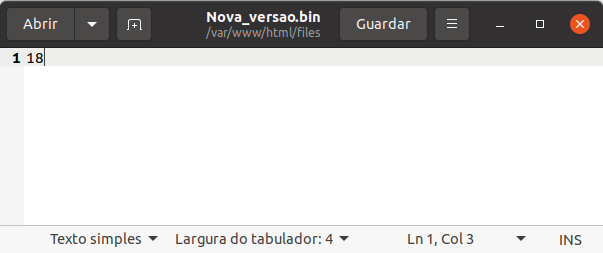
\includegraphics[scale=0.9]{dados/figuras/arquivodeversao.png}
     \caption{Arquivo de versão que somente contém o numero da versão.\newline Fonte: autoria própria.}
     \label{arquivoversao}
\end{figure}

O arquivo contendo a hash do firmware deve ser obtido a partir da função de hash criptográfico SHA-256, em sistemas linux essa função pode ser obtida pelo comando "sha256sum" como demonstrado na \autoref{gerandohash}. Este dado deve ser salvo em modo texto também, como também é possível ser observado na \autoref{gerandohash}.

\begin{figure}[H]
    \scriptsize
     \centering
     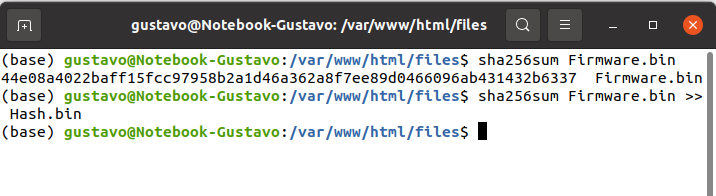
\includegraphics[scale=0.8]{dados/figuras/hashcreate.png}
     \caption{Criação de um novo arquivo contendo o hash do \firmware.\newline Fonte: autoria própria.}
     \label{gerandohash}
\end{figure}
\subsection{CRIAÇÃO DE FIRMWARE PARA ATUALIZAÇÃO}
O arquivo contendo o \firmware\ deve ser um binário gerado pelo compilador 

\subsection {FIRMWARES DE TESTE PROPOSTOS}
Para os testes apresentados neste trabalho foram desenvolvidos dois \textit{firmwares} muito parecidos, ambos possuem todas as bibliotecas necessárias para que o sistema de atualização OTA proposto funcione corretamente, além de possuírem o sistema operacional de tempo real FreeRTOS. Esses \textit{firmwares} foram desenvolvido para somente darem suporte ao sistema e não exercerem nenhuma outra função, com isso temos uma estimativa do tamanho que somente o sistema de atualização, suas bibliotecas e o FreeRTOS ocupam em memória.

Esses \textit{firmwares} contém além de inicializações necessárias de drivers, bibliotecas e do sistema operacional, uma pequena função que apresenta uma mensagem de apresentação mostrando a versão do \firmware\ atual e uma mensagem de teste somente para fazer uma diferenciação entre as versões, as frases são \textit{"Firmware 1 - Technology is just nature we taught to do cool trick"} e \textit{"Firmware 2 - The universe is a complexity machine"}. A mensagem de boas vindas do \firmware\ 1 pode ser observado na \autoref{mensagemteste1} e a do \firmware\ 2 na \autoref{mensagemteste2}. 

\begin{figure}[H]
    \scriptsize
     \centering
     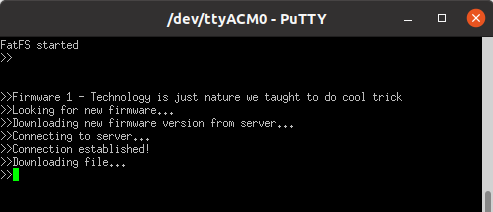
\includegraphics[scale=1]{dados/figuras/mensagem1.png}
     \caption{Mensagem de boas vindas do \firmware\ 1. \newline Fonte: Autoria própria.}
     \label{mensagemteste1}
\end{figure}
\begin{figure}[H]
    \scriptsize
     \centering
     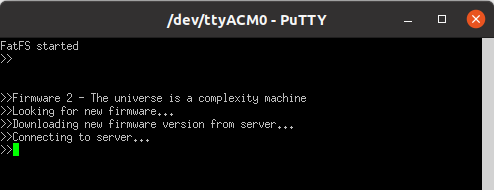
\includegraphics[scale=1]{dados/figuras/mensagem2.png}
     \caption{Mensagem de boas vindas do \firmware\ 2. \newline Fonte: Autoria própria.}
     \label{mensagemteste2}
\end{figure}

A função padrão destes firmware é um laço infinito que a cada 1 segundos inicializa a função OTA que realiza o processo de atualização, assim temos uma garantia que o firmware ira sempre ficar executando a função OTA.


\section{MATERIAIS UTILIZADOS}

A API e o bootloader foram escritos na linguagem C, enquanto o \linker\ será escrito em comandos de \linker. A escrita desses códigos será feita com o uso do ambiente de desenvolvimento integrado Eclipse \cite{Eclipse}. O sistema de atualização OTA desenvolvido nesse trabalho é inicialmente desenvolvido para a plataforma STM32F746G-Discovery.

\subsection{PLATAFORMA STM32F746G-DISCOVERY}

O STM32F7 Discovery é um kit de desenvolvimento que permite ao usuário desenvolver e compartilhar aplicações com toda a série de microcontroladores STM32F7 baseados no processador ARM\textregistered  Cortex\textregistered-M7 core.
O kit discovery permite uma ampla diversidade de aplicações que podem se beneficiar de suporte a múltiplos sensores, áudio, tela gráfica, segurança, vídeos e conexões de alta velocidade \cite{STM32F7}.
A \autoref{STM32F7} ilustra o kit STM32F746NGH6-Discovery.

\begin{figure}[H]
    \scriptsize
     \centering
     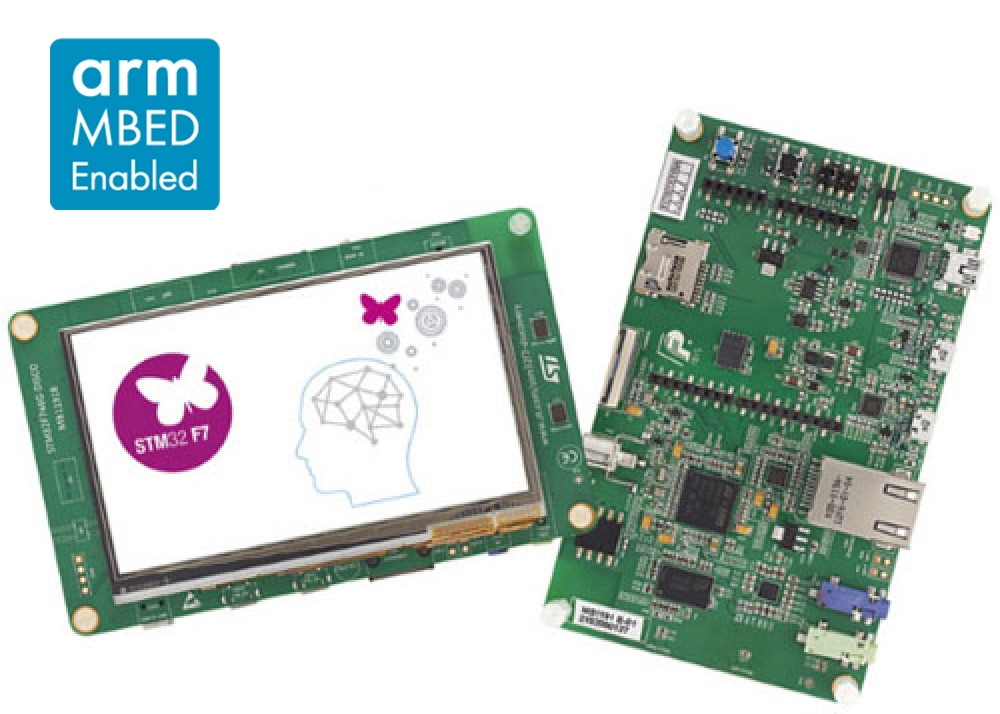
\includegraphics[scale=0.4]{dados/figuras/STM32F7.jpg}
     \caption{Kit de desenvolvimento STM32F746G-Discovery. \newline Fonte:\cite{STM32F7}.}
     \label{STM32F7}
\end{figure}

Algumas de suas principais características são \cite{STM32F7}:
\begin{itemize}
    \item Microcontrolador STM32F746NGH6 com 1 Mbytes de memória flash e 340 Kbytes de RAM, em um pacote BGA216.
    \item 128-Mbit de memória Quad-SPI Flash.
    \item 128-Mbit SDRAM (Com 64 Mbits Acessível).
    \item Conector para cartão microSD.
    \item Conector Ethernet em conformidade com a IEEE-802.3-2002
    \item Tela LCD de 4,3 polegadas, com resolução de 480x272 com \textit{touch-screen} capacitivo.
    
\end{itemize}
\section{UTILIZANDO O SISTEMA}
Com o intuito de fazer a ferramenta criada neste projeto ser facilmente utilizada por diversos desenvolvedores essa sessão foi criada para facilitar o entendimento de como utilizar o sistema de atualização OTA proposto. Destacando como portar e utilizar o \bootloader\ e toda a API do firmware OTA. Para a utilização de ambos os programas desenvolvidos neste trabalho é sempre necessário que as bibliotecas que são utilizadas por eles já estejam incluídas no projeto. Para o \bootloader, é necessário somente a biblioteca FATFS, enquanto para o OTA são necessárias as bibliotecas FATFS, LWIP e MBED TLS.

\subsection{PORTANDO O BOOTLOADER}
Para se utilizar o \bootloader proposto em outros sistemas embarcados da familia STM32 deve-se primeiramente observar a organização da memória FLASH do sistema microcontrolado que se deseja portar o \bootloader. Como podemos observar na \autoref{STM32F7_FLASH} a memória FLASH do microcontrolador STM32F746NGH6 possui oito setores de memória com tamanhos distintos, com isso foi selecionado o primeiro setor de memória para abrigar o \bootloader.

\begin{table}[H]
    \scriptsize
    \centering
    \begin{tabular}{|c|c|c|}

    \hline
    Nome    & Endereço do bloco         & Tamanho do setor \\ \hline
    Setor 0 & 0x0800 0000 - 0x0800 7FFF & 32 Kbytes        \\ \hline
    Setor 1 & 0x0800 8000 - 0x0800 FFFF & 32 Kbytes        \\ \hline
    Setor 2 & 0x0801 0000 - 0x0801 7FFF & 32 Kbytes        \\ \hline
    Setor 3 & 0x0801 8000 - 0x0801 FFFF & 32 Kbytes        \\ \hline
    Setor 4 & 0x0802 0000 - 0x0803 FFFF & 128 Kbytes       \\ \hline
    Setor 5 & 0x0804 0000 - 0x0807 FFFF & 256 Kbytes       \\ \hline
    Setor 6 & 0x0808 0000 - 0x080B FFFF & 256 Kbytes       \\ \hline
    Setor 7 & 0x080C 0000 - 0x080F FFFF & 256 Kbytes       \\ \hline
    \end{tabular}
    \caption{Organização do bloco de memória FLASH do microcontrolador STM32F746NGH6. \newline Adaptado de:\cite{STM32F7}.}
    \label{STM32F7_FLASH}
    \end{table}


Para fazer o porte foi necessário modificar no arquivo de linker o tamanho máximo da memória utilizável para evitar que os dados do \bootloader\ ultrapassem o tamanho que determinamos para ele. Assim no arquivo de linker foi modificado de forma que o tamanho máximo da memória seja de 32 Kbytes e iniciada no setor 0. Com isso a configuração de memória do \bootloader\ para o microcontrolador utilizado neste trabalho ficou da seguinte forma:


\begin{algorithm}[H]
\begin{lstlisting}
/* Specify the memory areas */
MEMORY
{
RAM (xrw)      : ORIGIN = 0x20000000, LENGTH = 320K
FLASH (rx)      : ORIGIN = 0x8000000, LENGTH = 32K
}

\end{lstlisting}
\caption{Trecho do arquivo de comandos de linker que é necessário alterar para o porte do \textit{bootloader}.
\newline Fonte: Autoria própria.}
\end{algorithm}

Como cada microcontrolador tem sua configuração de memória, o desenvolvedor deve observar a configuração do sistema alvo e colocar sempre o \bootloader no setor 0 de seu microcontrolador.

Feita a modificação no arquivo de linker, o desenvolvedor iniciará a alteração do arquivo \textbf{bootloader.h} que contém algumas definições dependentes do seu microcontrolador. Neste arquivo as definições que precisam ser alteradas são:
\begin{itemize}
    \item FIRMWARE\_VERSION\_ADDRESS: Esta definição mostra ao \bootloader\ a posição na memória FLASH em que se deve armazenar a versão atual da aplicação presente na placa, deve ser sempre os quatro últimos bytes da memória, e necessita sempre ser a mesma posição configurada na API de atualização OTA. No caso do microcontrolador deste trabalho foi utilizada a posição: 0x080FFFFC.
    \item FIRMWARE\_PATH: Esta definição mostra qual o caminho do arquivo em que se encontra o novo firmware que foi baixado pela API OTA, deve ser sempre igual ao que será definido na API.
    \item FIRMWARE\_NEW\_VERSION\_PATH: Esta definição mostra qual o caminho do arquivo em que se encontra a versão do novo firmware que foi baixado pela API OTA, deve ser sempre igual ao que será definido na API.
    \item APP\_START\_ADDRESS: Esta definição mostra ao \bootloader\ a posição na memória FLASH em que se deve armazenar o inicio da aplicação que será trocada sendo sempre o inicio do setor 1. No caso do microcontrolador deste trabalho foi utilizada a posição: 0x08008000.
   
\end{itemize}

Com essas alterações já é possível utilizar o \bootloader\ em sistemas embarcados que utilizam microcontroladores da família STM32, restando agora a configuração da API de atualização OTA que será utilizada em conjunto com o \bootloader.

\subsection{CONFIGURAÇÃO DA API OTA}
Assim como no \bootloader, a aplicação também precisa ter seu arquivo de linker modificado para evitar sobrescritas no espaço reservado para o \bootloader\ e reservar o espaço necessário para a variável de versão. Com isso o desenvolvedor deve novamente observar a \autoref{STM32F7_FLASH} e verificar qual posição de memória se inicia sua aplicação e o tamanho total dela deve ser obtido com a seguinte formula:

\begin{equation}
    Tamanho\ do\ app = Final\ da\ FLASH - inicio\ do\ setor\ 1\ da\ FLASH - 4\ bytes 
    \label{eq:calculo_flash}
\end{equation}


Utilizando a formula para o microcontrolador STM32F746NGH6 temos que o inicio do setor 1 de memória é 0x08008000 e o fim do ultimo setor de memória é 0x080FFFFF, assim podemos obter os valores de de inicio e tamanho da aplicação e assim configurar o arquivo de linker da aplicação da seguinte forma:


\begin{algorithm}[H]
\begin{lstlisting}
/* Specify the memory areas */
MEMORY
{
RAM (xrw)      : ORIGIN = 0x20000000, LENGTH = 320K
FLASH (rx)      : ORIGIN = 0x08008000, LENGTH = 0xF7FFB
}
\end{lstlisting}
\caption{Trecho do arquivo de comandos de linker que é necessário alterar para o porte da aplicação.
\newline Fonte: Autoria própria.}
\end{algorithm}

Feitas as alterações necessárias no arquivo de linker, o desenvolvedor tem que alterar algumas definições no arquivo \textbf{ota\_server.h} com o intuito de adequar a API de atualização OTA para a sua aplicação. Neste arquivo as definições que precisam ser alteradas são:

\begin{itemize}
    \item FIRMWARE\_VERSION\_ADDRESS: Esta definição mostra a aplicação a posição na memória FLASH em que se deve armazenar a versão atual da aplicação presente na placa e deve ser sempre os quatro últimos bytes da memória, e deve sempre ser o mesmo configurado no \bootloader. No caso do microcontrolador deste trabalho foi utilizada a posição: 0x080FFFFC.
    \item FIRMWARE\_PATH: Esta definição mostra qual o caminho do arquivo em que de deve armazenar o novo \firmware\ que deverá ser baixado pela API OTA, deve ser sempre igual ao que será definido no \bootloader.
    \item FIRMWARE\_NEW\_VERSION\_PATH: Esta definição mostra qual o caminho do arquivo em que se deve armazenar a versão do novo \firmware\ que será baixado pela API OTA, deve ser sempre igual ao que será definido no \bootloader.
    \item BOOTLOADER\_START\_ADDRESS: Esta definição mostra a aplicação a posição na memória FLASH em que está armazenado o inicio do \bootloader sendo sempre o inicio do setor 0. No caso do microcontrolador deste trabalho foi utilizada a posição: 0x08000000.
    \item FIRMWARE\_NEW\_VERSION\_HASH\_PATH: Esta definição mostra qual o caminho do arquivo em que de deve armazenar o hash do novo \firmware\ para que se compare com o hash gerado pelo \firmware\ baixado, assim fazendo um teste para verificar se o \firmware\ baixado é integro e autentico.
    \item AUTH\_SERVER: Esta definição mostra qual deve ser o endereço do servidor em que se deve obter os arquivos necessários para a atualização de \firmware, então deve ser personalizada para cada aplicação.
    \item AUTH\_PORT: Esta definição mostra qual deve ser a porta que se deve conectar no servidor, como estamos utilizando uma camada de TLS esta porta deve ser a 443.
    \item AUTH\_REQUEST\_VERSION: Esta definição mostra qual a requisição HTTP do arquivo contendo o número da nova versão que deverá ser baixada pela API.
    \item AUTH\_REQUEST\_FIRMWARE: Esta definição mostra qual a requisição HTTP do firmware da nova versão que deverá ser baixada pela API.
    \item AUTH\_REQUEST\_HASH: Esta definição mostra qual a requisição HTTP do arquivo contendo o hash da nova versão que deverá ser baixada pela API.
    \item SSL\_CA\_PEM: Esta definição mostra o certificado SSL utilizado na comunicação com o servidor.
\end{itemize}

Com essas definições corretamente configuradas pode-se utilizar facilmente a API de atualização OTA proposta neste trabalho, ficando a cargo do desenvolvedor somente programar em sua aplicação o algoritmos que determina quando a função que inicia a atualização é chamada, para que o processo de atualização OTA proposto neste trabalho se encarregue de fazer todo o processo de forma autónoma. 

